\documentclass{article}
\usepackage{amsmath}
\usepackage{amssymb}
\usepackage{graphicx}
\usepackage{hyperref}
\usepackage[version=4]{mhchem}

\title{Example 4}
\date{}

\begin{document}
\maketitle

\(A B\) is the diameter of circle \(O . C\) is a point on the circumference of circle \(O . A D\) is perpendicular to the tangent line drawn through \(C\). Show that \(A C\) is the angle bisector of \(\angle D A B\).

Solution:
Method 1:\\
\centering
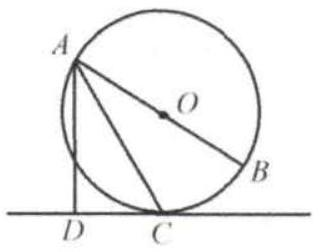
\includegraphics[width=\textwidth]{images/164(1).jpg}

Connect \(C B\).\\
Since \(A B\) is the diameter, \(\angle A C B=90^{\circ}\).\\
Since \(A D \perp D C, \angle A D C=90^{\circ}\).\\
\(\angle A C D=\angle A B C\) (they face the same arc \(A C\) ).\\
Thus \(\triangle A C D \sim \triangle A B C\).\\
So \(\angle D A B=\angle C A B\).\\
\(A C\) is the angle bisector of \(\angle D A B\).\\
\centering
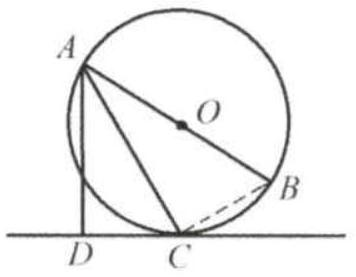
\includegraphics[width=\textwidth]{images/164(2).jpg}

Method 2:\\
Connect \(C B\).\\
Since \(A B\) is the diameter, \(\angle A C B=90^{\circ}\).\\
So \(\angle 3+\angle 4=90^{\circ}\).\\
\(\angle 3=90^{\circ}-\angle 4\).\\
Since \(A D \perp D C, \angle 1+\angle 4=90^{\circ}\).\\
\(\angle 1=90^{\circ}-\angle 4\).\\
\(\angle 1=\angle 3\).\\
\centering
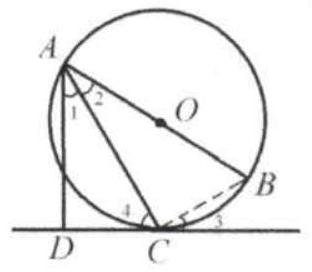
\includegraphics[width=\textwidth]{images/164(3).jpg}\\
\(\angle 3=\angle 2\) (they face the same arc \(A C\) ).\\
Thus \(\angle 1=\angle 2\).\\
\(A C\) is the angle bisector of \(\angle D A B\).



\end{document}
